
%That is, a system $(B, Q_0)$ whose set of states is finite. 
%Implementations of the method for infinite-state systems are a subject for future work.
\ldfctool, ($\sim 1500$ LOC Java) implements our method for finite-state BIP-systems.
Pseudocode for \ldfctool is shown in Figure~\ref{fig:implementation}.
%
\checkLin{$\B, Q_0$}\ iterates over each interaction $\act$ of ($\B, Q_0$), and checks 
$(\ex \l > 0: \LLin(B, Q_0, \act, \l))$ by starting with $\l=1$ and incrementing $\l$ until
either $\LLin(B, Q_0, \act, \l)$ is found to hold, or 
$\dsk{\act}{\l}$ has become the entire system and $\LLin(B, Q_0, \act, \l)$ does not hold. In the latter case, 
$\LLin(B, Q_0, \act, \l)$ does not hold for any finite $\l$, and, in practice, 
computation would halt 
before $\dsk{\act}{\l}$ had become the entire system, due to exhaustion of resources.

\checkLinIntDist{$\B, Q_0, \act, \l$} checks $\LLin(B, Q_0, \act, \l)$ by examining every reachable transition
that executes $a$, and checking that the final state satisfies
Definition~\ref{def:ldfc-k}. 


\paragraph{Complexity.} The running  time of our implementation is 
$O(\SUM_{a \in \gamma} |\dsk{\act}{\l_a}|)$, where $\l_a$ is the smallest value
of $\l$ for which $\LLin(\act, \l)$ holds, and where
$|\dsk{\act}{\l_a}|$ denotes the size of the transition system of $\dsk{\act}{\l_a}$.

%If $\LDFC(a, \l)$ does not hold for any finite $\l$, then the
%iteration for $a$ must be halted by some predetermined time bound, or
%interactively, or when $\dsk{\act}{\l}$ has become the entire system.




\begin{figure}[ht]

\setcounter{lctr}{0}
\begin{tabbing}\label{alg:check-df}
mm\= mm\= mm\= \kill
\checkLin{$\B, Q_0$},  where $\B \df \gamma(\B_1,\dots,\B_n)$\\
\lio{\FORALLC{\mbox{interactions $\act \in \gamma$}}}
   \lit{\IFC{\checkLinInt{\B, Q_0, \act} = \fff}\ \RETURNE{\fff} \ \FI}
\lio{\ENDFOR;}
\liocn{\RETURNE{\ttt}}{\cmnt\ return $\ttt$ if check succeeds for all $\act \in \gamma$}
\end{tabbing}

\setcounter{lctr}{0}
\begin{tabbing}\label{alg:checkInt}
mm\= mm\= mm\= \kill
\checkLinInt{$\B, Q_0, \act$},  where $\B \df \gamma(\B_1,\dots,\B_n), \act \in \gamma$\\
\cmnt\ check $(\ex \l > 0: \LLin(\B, Q_0, \act, \l))$\\
\lioc{\l \gts 1;}{\cmnt\ start with $\l = 1$}
\lio{\WHILEC{\ttt}}
   \litc{\IFC{\checkLinIntDist{\act, \l} = \ttt}\ \RETURNE{\ttt}\ \FI;}{\cmnt\ success, so return true}
   \litc{\IFC{\dsk{\act}{\l} = \gamma(\B_1,\dots,\B_n)}\ \RETURNE{\fff}\ \FI;}{\cmnt\ exhausted all subsystems, return false}
   \litc{\l \gts \l + 1}{\cmnt\ increment $\l$ until success or intractable or failure}
\lio{\ENDWHILE}
\end{tabbing}

\setcounter{lctr}{0}
\begin{tabbing}
\label{alg:eval-ldfc}
mm\= mm\= mm\= \kill
\checkLinIntDist{$\B, Q_0, \act, \l$}\\
\lio{\FORALLC{\mbox{reachable transitions $s_\act \goesto[\act] t_\act$ of $\dsk{\act}{\l}$}}}
   \lit{\IFC{\neg(\fa \B_i \in \cmps{\act}:  \widepth{\dsk{\act}{\l}}{\B_i}{t_\act} < 2\l - 1 \lor \wodepth{\dsk{\act}{\l}}{\B_i}{t_\act} < 2\l -1)}}
  	\lihc{\RETURNE{\fff}}{\cmnt\ check Definition~\ref{def:ldfc-k}}
  \lit{\FI}
\lio{\ENDFOR;}
\liocn{\RETURNE{\ttt}}{\cmnt\ return $\ttt$ if check succeeds for all transitions}
\end{tabbing}

\caption{Pseudocode for the implementation of the linear condition.}
\label{fig:implementation}
\label{fig:implementation-checkDF}
\end{figure}




\subsubsection{Experiment: Dining Philosophers} 
We consider $n$ philosophers in a cycle, based on the components of Figure~\ref{fig:diningSpectrum}.
Figure~\ref{bench:dining} provides experimental results.
The $x$ axis gives the number $n$ of philosophers (and also the number of forks), 
and the $y$ axis gives the verification time (in
milliseconds).  We verified that $\LDFC(a, \l)$ holds for
$\l = 1$ and all interactions $a$. Hence dining philosophers is deadlock-free.
%
We increase $n$ and plot the verification
time for both \ldfctool and D-Finder 2~\cite{DFinder2}.
D-Finder 2 implements a compositional and incremental method for the
verification of BIP-systems. D-Finder
(the precursor of D-Finder 2) has been compared favorably with NuSmv and
SPIN, outperforming both  NuSmv and SPIN on
dining philosophers, and outperforming NuSmv on the gas station
example~\cite{bensalem2010compositional}, treated next.
%
Our results show that \ldfctool has a linear increase of computation time with the system size
$(n)$, and so outperforms D-Finder 2.


\subsubsection{Experiment: Gas Station}
A gas station \cite{gasstation} consists of an operator, % with a computer,
a set of pumps, and a set of customers. 
%Each pump can be used by a fixed number of customers.
Before using a pump, a customer has to prepay. Then the customer uses the
pump, collects his change and %goes to a state from which he may start
starts a new transaction.
%
Before being used by a customer, a pump has to be activated by the
operator.  When a pump is shut off, it can be re-activated for the
next operation.  


Figure \ref{fig:gas-station} gives the model for a
gas station system for one pump and two customers.  The operator has
two control locations and three ports. The transition labeled with
$\mathit{prepay}$ accepts a customer's prepay and activates the pump for the
customer. When a customer is served, the transition labeled with
$\mathit{finish}$ synchronizes the pump and the customer.  A pump has three
control locations and three ports. Besides the synchronization between
the operator and customer through activate and finish ports, a pump
and a customer are synchronized through $\mathit{start}$ ports.

\begin{figure}[ht]
\begin{center}
\scalebox{0.5}{\input{figs/gas_station.pdf_t}}
\caption{Sketch of Gas Station}
\label{fig:gas-station}
\end{center}
\end{figure}


We verified $\LDFC(\B, Q_0, \act, \l)$ for $\l=2$ and all interactions $a$.
Hence gas station is deadlock-free.  Figures~\ref{bench:gasstation1},
\ref{bench:gasstation2}, and \ref{bench:gasstation3} present the verification
times using \ldfctool and D-Finder 2. We consider a system with 3 pumps and variable number
of customers.  In these figures, the $x$ axis gives the number $n$ of
customers, and the $y$ axis gives the verification time (in seconds).
%
D-Finder 2 suffers state-explosion at $n = 1800$,
because we consider only three pumps, and so the incremental method used by
D-Finder 2 deteriorates. \ldfctool outperforms D-Finder 2 as the number of
customers increases.


\begin{figure}[t]
  \begin{center}
    \mbox{
       \hspace*{-0.5cm}\subfigure[Dining philosophers benchmark.]{\label{bench:dining}\scalebox{0.24}{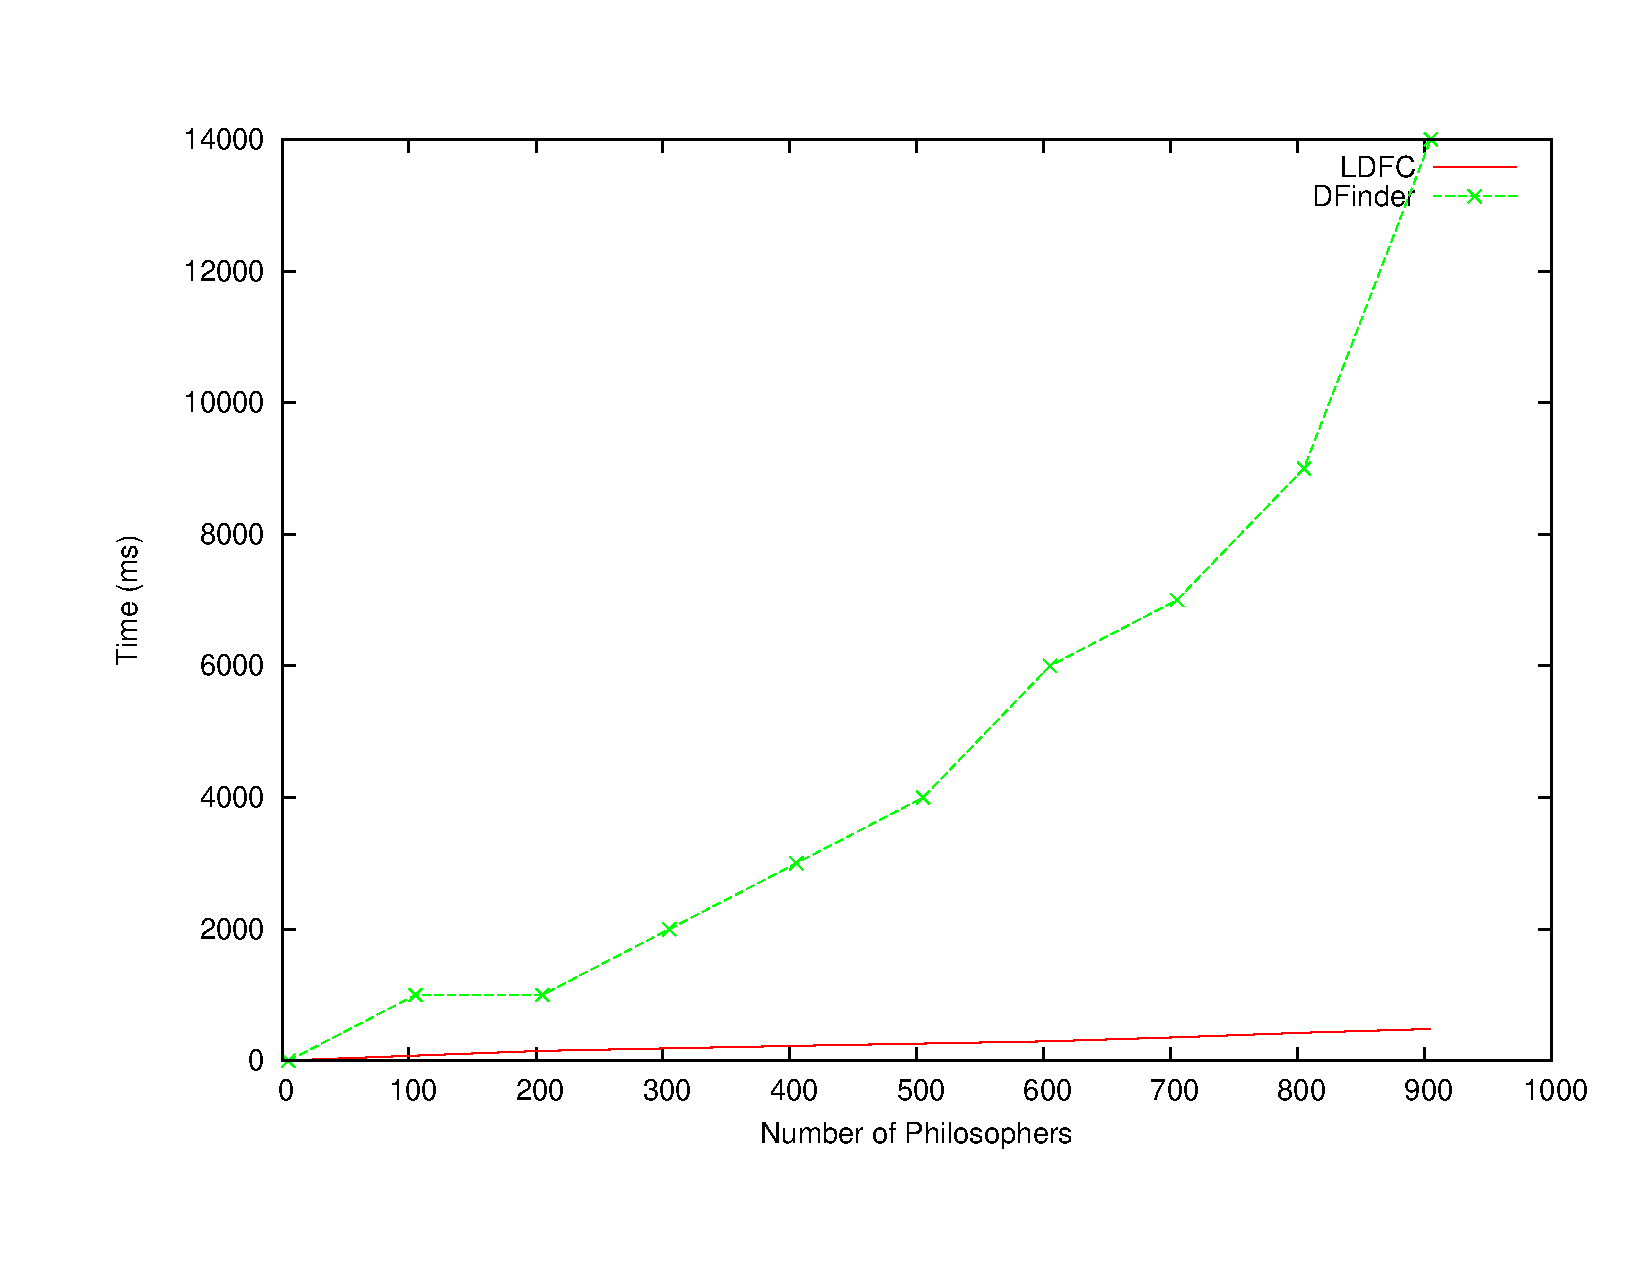
\includegraphics{figs/bench.pdf}}} 
       \hspace*{-0.7cm}\subfigure[Gas station benchmark 1.]{\label{bench:gasstation1}\scalebox{0.24}{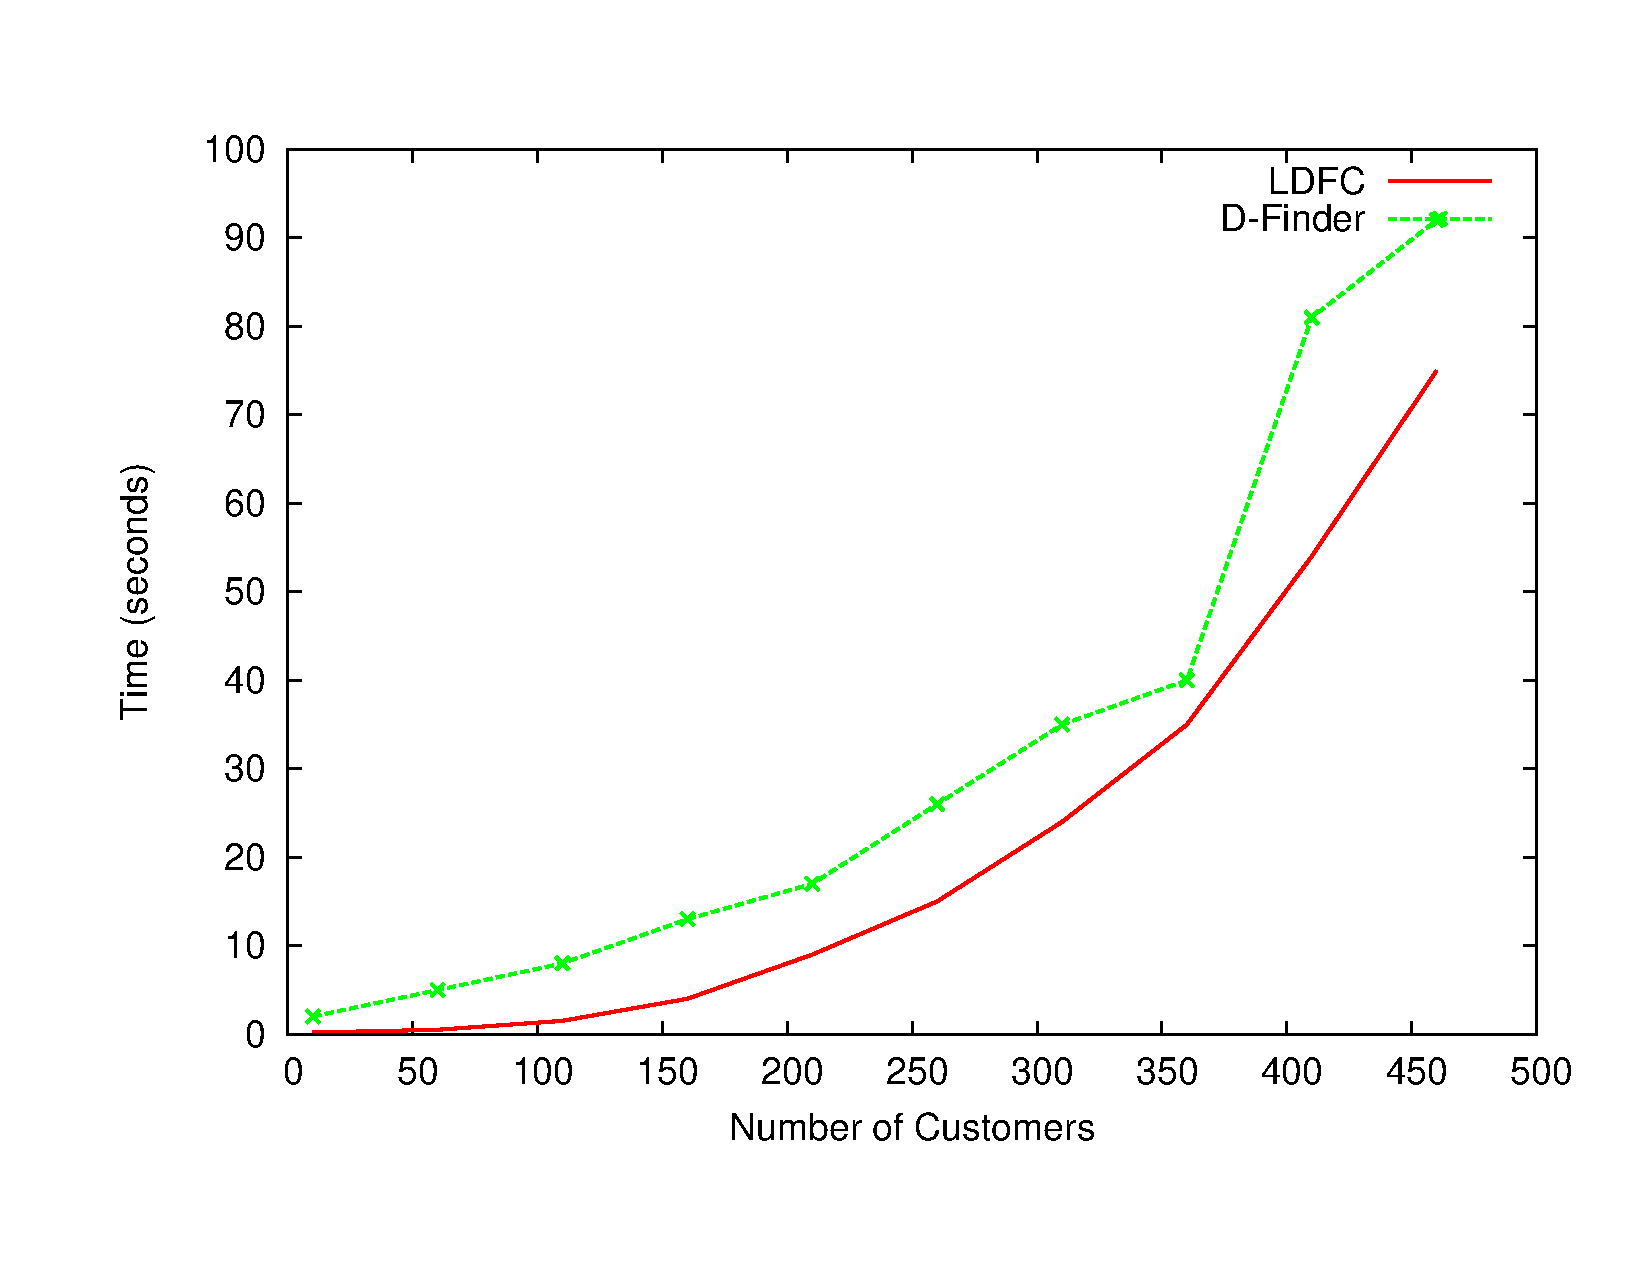
\includegraphics{figs/benchgas1.pdf}}} 
      }\vspace*{0.05cm}
     \mbox{
        \hspace*{-0.6cm} \subfigure[Gas station benchmark 2.]{\label{bench:gasstation2}\scalebox{0.24}{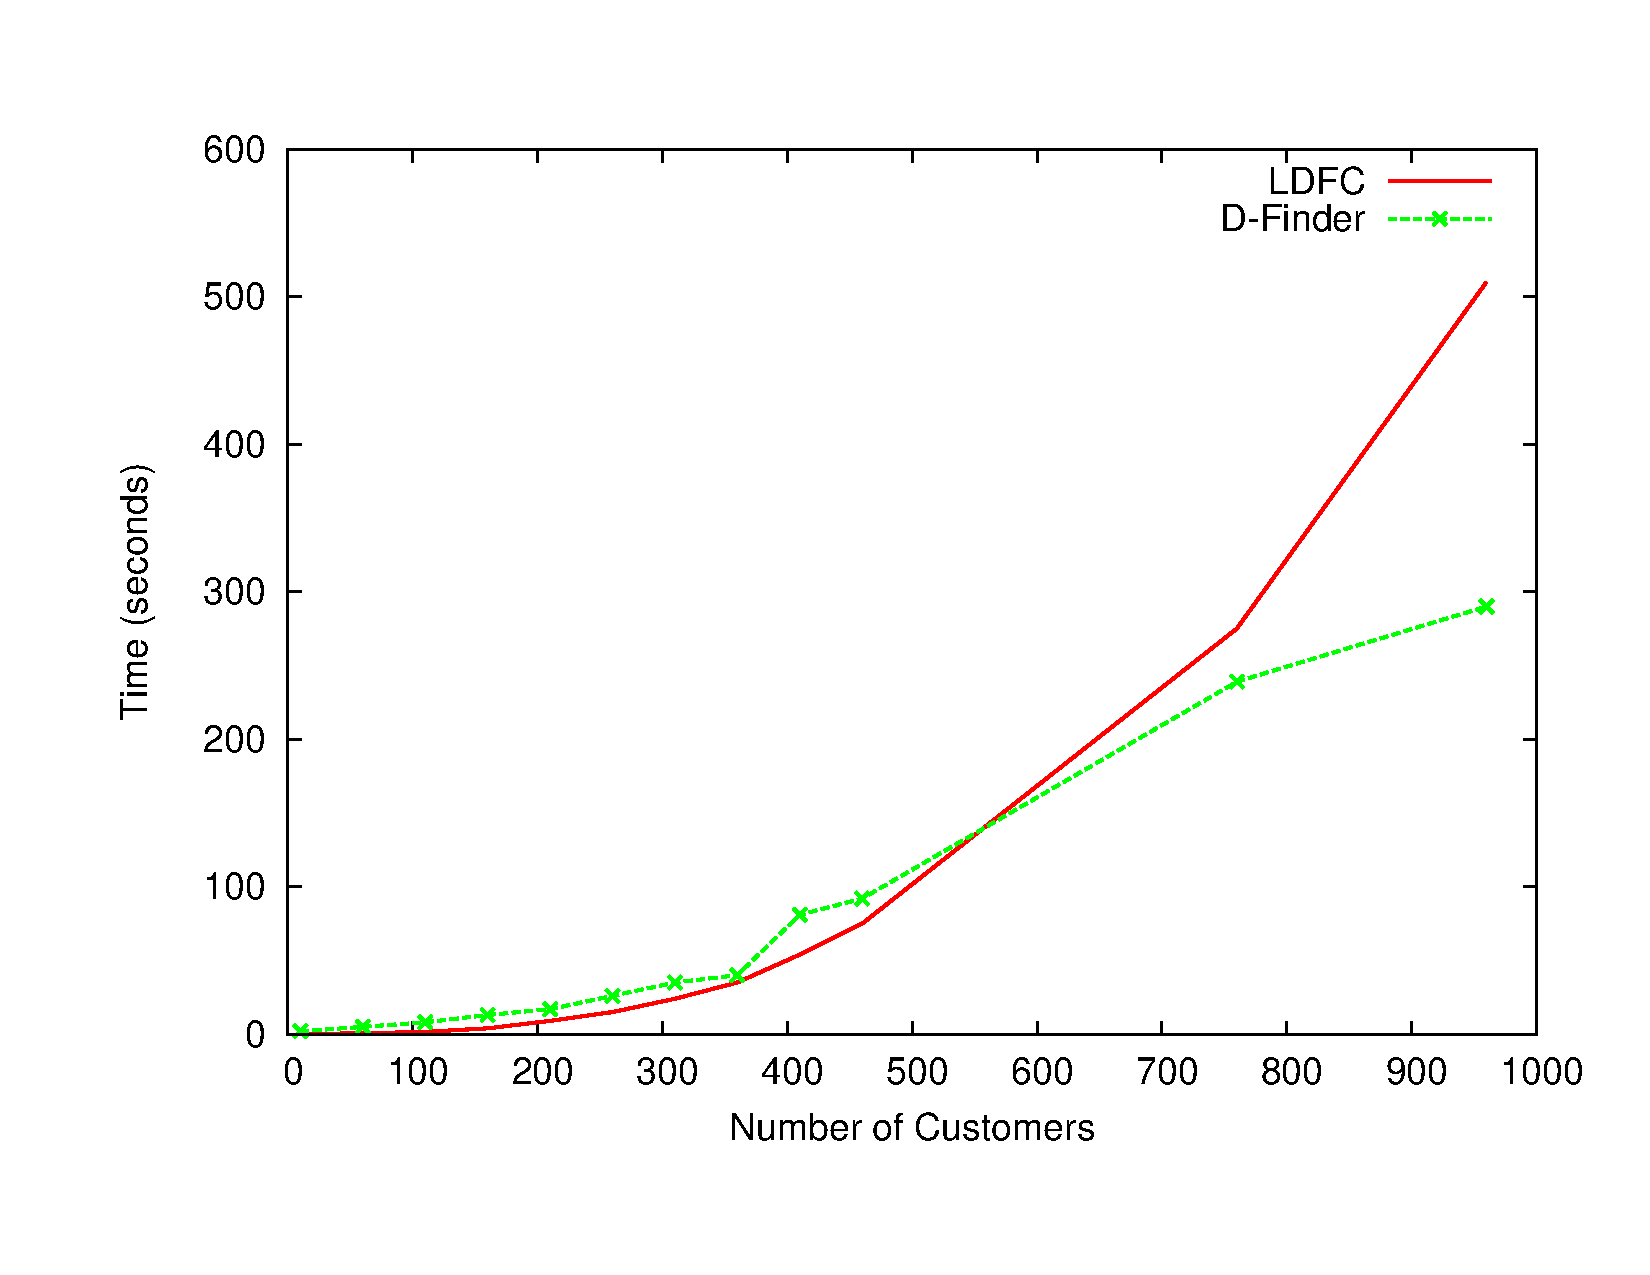
\includegraphics{figs/benchgas2.pdf}}} 
        \hspace*{-0.7cm} \subfigure[Gas station benchmark 3.]{\label{bench:gasstation3}\scalebox{0.24}{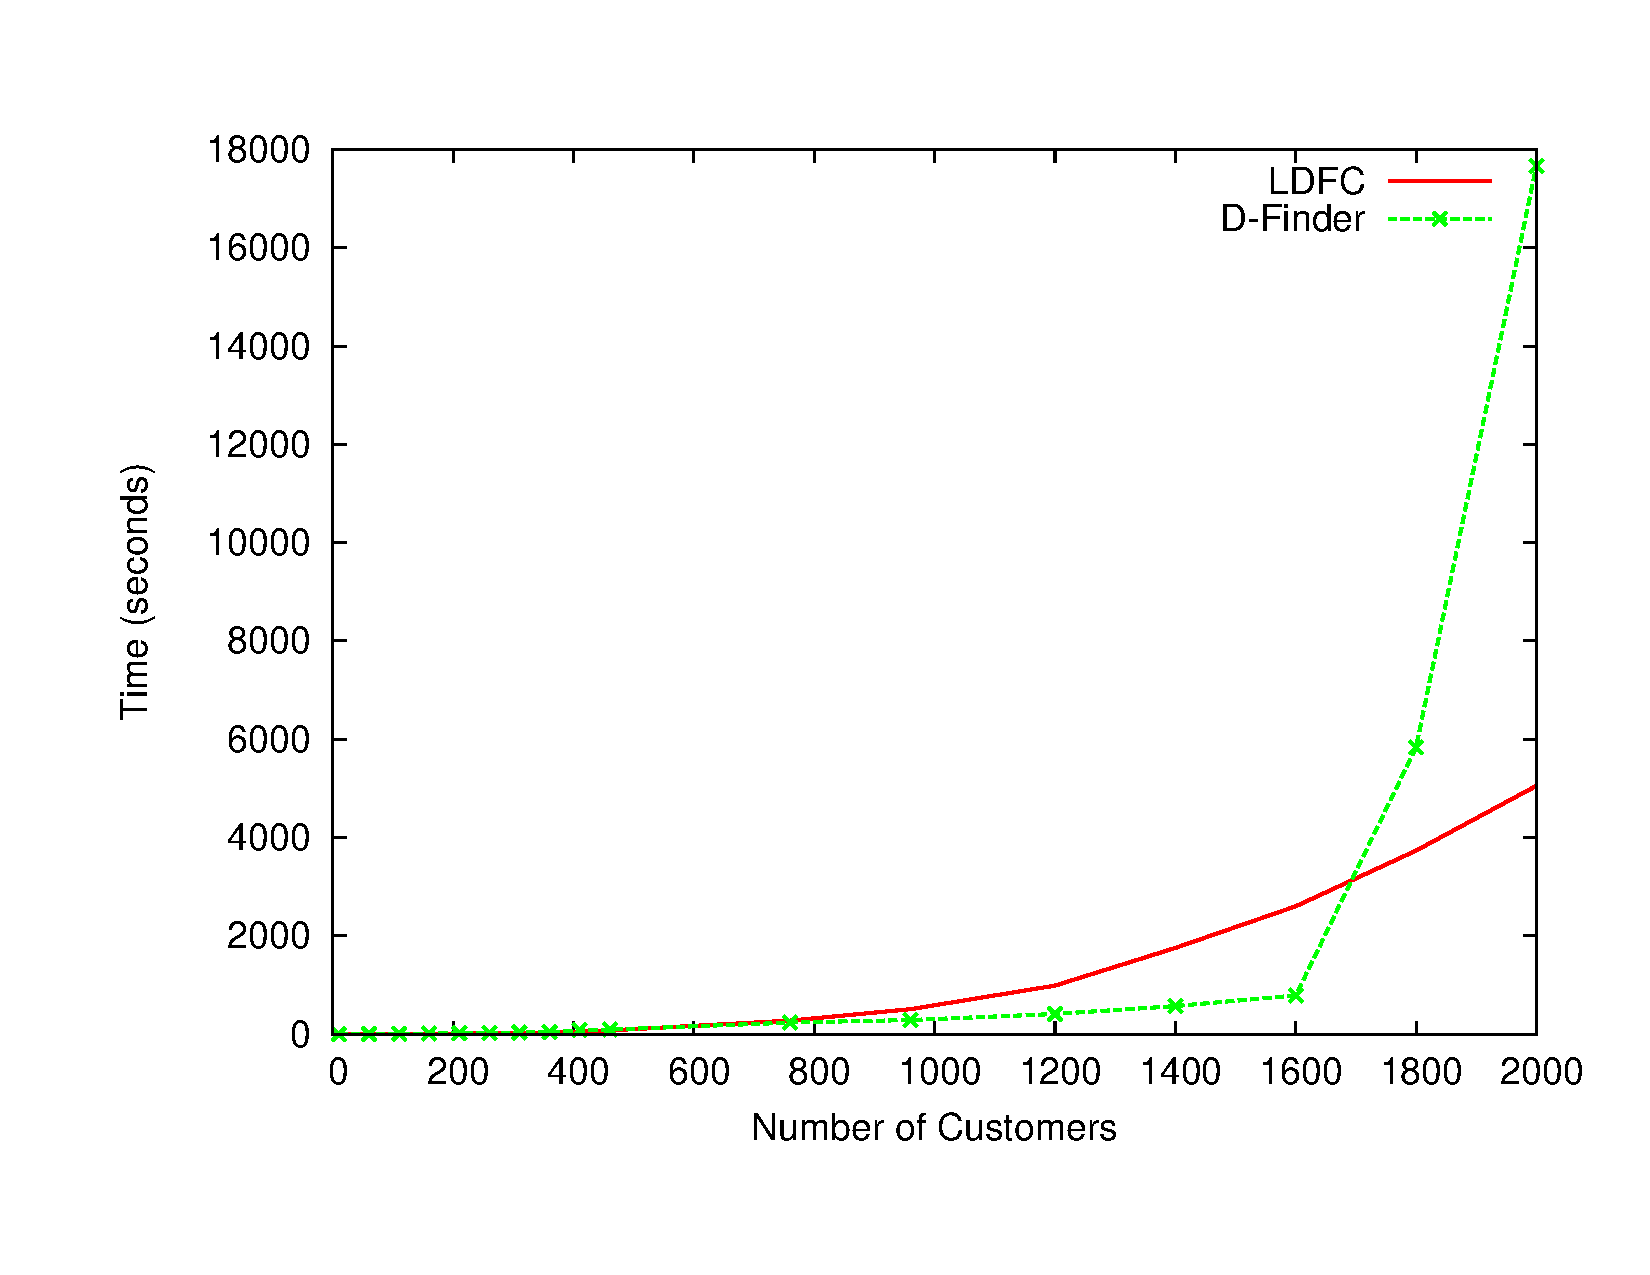
\includegraphics{figs/benchgas3.pdf}}}
      }\vspace*{-0.2cm}
    \caption{Benchmarks generated by our experiments.}
    \label{fig:gasSpectrum}
  \end{center}
\end{figure}


